\documentclass[varwidth]{standalone}
\usepackage[portrait,paperwidth=30cm,
paperheight=40cm,
textwidth=26cm,
textheight=36cm]{geometry}
\usepackage{bera}
\usepackage[T1]{fontenc}
\usepackage[swedish]{babel}
\usepackage[utf8]{inputenc}
\usepackage{amsmath}
\usepackage{bm}
\usepackage{tikz}
\usepackage{pgfplots}
\usepackage{tikz}
\usepackage{tkz-euclide}
\usepackage{pgfgantt}
\usetikzlibrary{decorations.pathmorphing}
\usetikzlibrary{patterns}
\usetikzlibrary{arrows}
\usepackage{pgfplots}
\usepackage{CJKutf8}
\pgfplotsset{compat=1.10}
\usetikzlibrary{shapes.geometric,arrows,fit,matrix,positioning}
\begin{document}
\newcommand{\radie}[0]{1mm}
\begin{center}
\begin{figure}
\centering
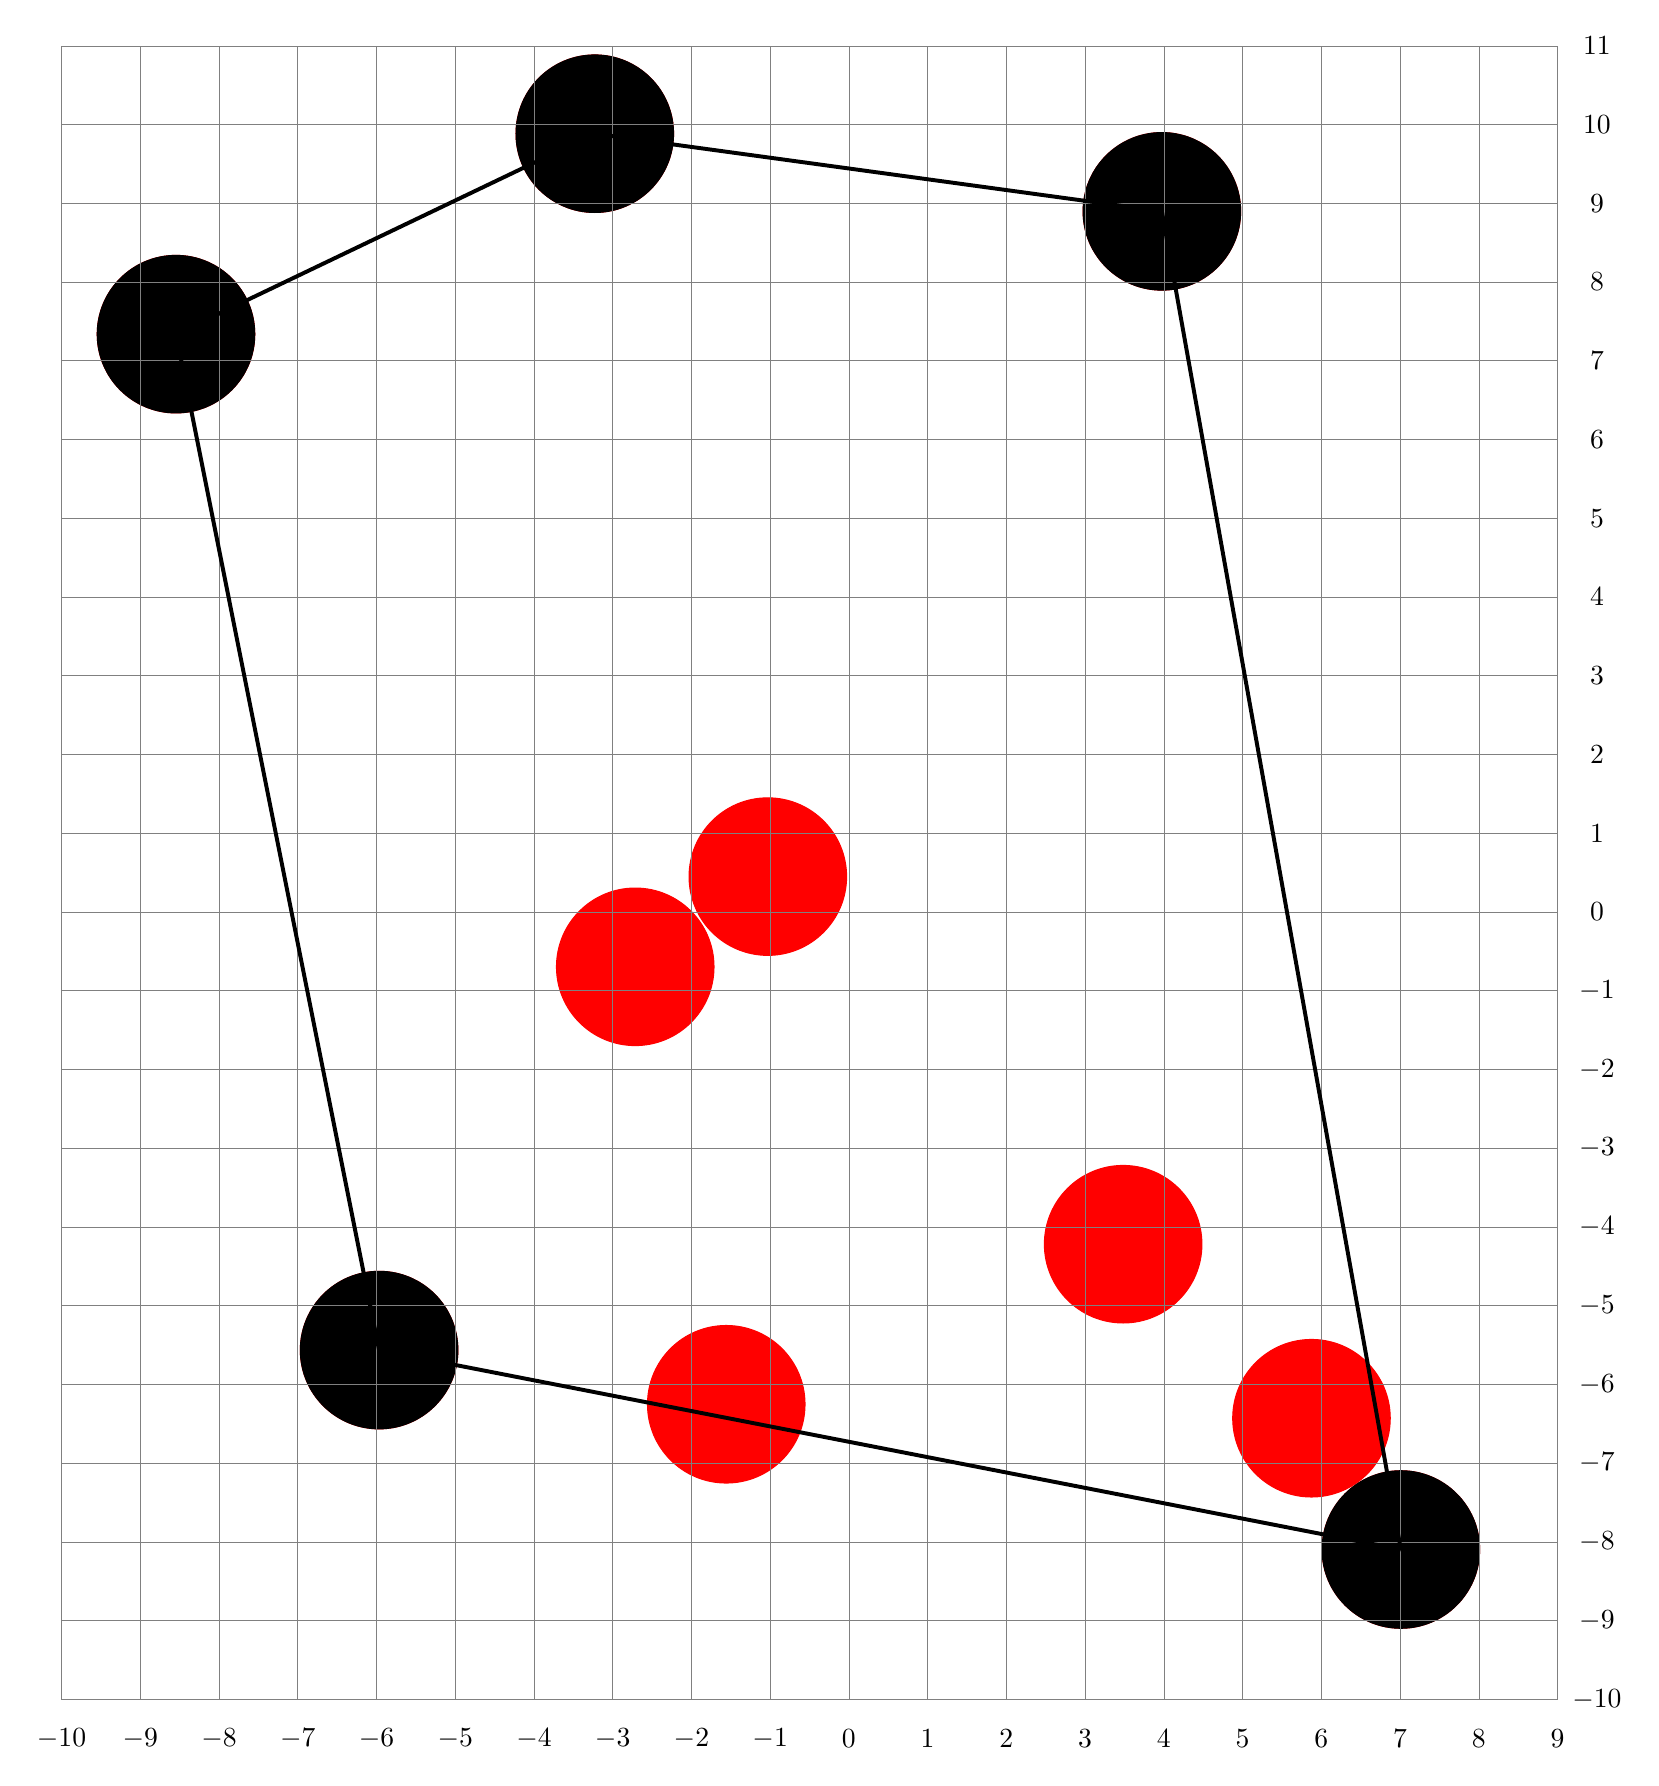
\begin{tikzpicture}
\draw [red,fill=red] (7.009764,-8.096763) circle(\radie);
\draw [red,fill=red] (3.483068,-4.219620) circle(\radie);
\draw [red,fill=red] (5.874824,-6.429663) circle(\radie);
\draw [red,fill=red] (-2.713367,-0.696560) circle(\radie);
\draw [red,fill=red] (-3.227101,9.883655) circle(\radie);
\draw [red,fill=red] (-5.966267,-5.564203) circle(\radie);
\draw [red,fill=red] (3.974697,8.897630) circle(\radie);
\draw [red,fill=red] (-1.029681,0.449005) circle(\radie);
\draw [red,fill=red] (-8.545768,7.337866) circle(\radie);
\draw [red,fill=red] (-1.557486,-6.252292) circle(\radie);
\draw [black,fill=black] (7.009764,-8.096763) circle(\radie);
\draw [black,fill=black] (-5.966267,-5.564203) circle(\radie);
\draw [black,fill=black] (-8.545768,7.337866) circle(\radie);
\draw [black,fill=black] (-3.227101,9.883655) circle(\radie);
\draw [black,fill=black] (3.974697,8.897630) circle(\radie);
\draw[step=10mm,gray,very thin] (-10,-10) grid (9,11);
\node at (-10,-10.500000) {$-10$};
\node at (-9,-10.500000) {$-9$};
\node at (-8,-10.500000) {$-8$};
\node at (-7,-10.500000) {$-7$};
\node at (-6,-10.500000) {$-6$};
\node at (-5,-10.500000) {$-5$};
\node at (-4,-10.500000) {$-4$};
\node at (-3,-10.500000) {$-3$};
\node at (-2,-10.500000) {$-2$};
\node at (-1,-10.500000) {$-1$};
\node at (0,-10.500000) {$0$};
\node at (1,-10.500000) {$1$};
\node at (2,-10.500000) {$2$};
\node at (3,-10.500000) {$3$};
\node at (4,-10.500000) {$4$};
\node at (5,-10.500000) {$5$};
\node at (6,-10.500000) {$6$};
\node at (7,-10.500000) {$7$};
\node at (8,-10.500000) {$8$};
\node at (9,-10.500000) {$9$};
\node at (9.500000,-10) {$-10$};
\node at (9.500000,-9) {$-9$};
\node at (9.500000,-8) {$-8$};
\node at (9.500000,-7) {$-7$};
\node at (9.500000,-6) {$-6$};
\node at (9.500000,-5) {$-5$};
\node at (9.500000,-4) {$-4$};
\node at (9.500000,-3) {$-3$};
\node at (9.500000,-2) {$-2$};
\node at (9.500000,-1) {$-1$};
\node at (9.500000,0) {$0$};
\node at (9.500000,1) {$1$};
\node at (9.500000,2) {$2$};
\node at (9.500000,3) {$3$};
\node at (9.500000,4) {$4$};
\node at (9.500000,5) {$5$};
\node at (9.500000,6) {$6$};
\node at (9.500000,7) {$7$};
\node at (9.500000,8) {$8$};
\node at (9.500000,9) {$9$};
\node at (9.500000,10) {$10$};
\node at (9.500000,11) {$11$};
\draw [line width = 0.5mm, black] (7.009764,-8.096763) -- 
(-5.966267,-5.564203) -- 
(-8.545768,7.337866) -- 
(-3.227101,9.883655) -- 
(3.974697,8.897630) -- 
(7.009764,-8.096763);
\end{tikzpicture}
\end{figure}
\end{center}
\end{document}
